\section{Major scale}
\begin{definition}[Tetrachord]
    A 4-note scale segment with the following steps: $W-W-H$.
\end{definition}

\begin{definition}[Major scale]
    A 8-note scale made up of 2 tetrachords, joined by a whole step.
\end{definition}

$$\underbrace{W-W-H}_{T1}-W-\underbrace{W-W-H}_{T2}$$

\begin{figure}[h]
    \begin{center}
        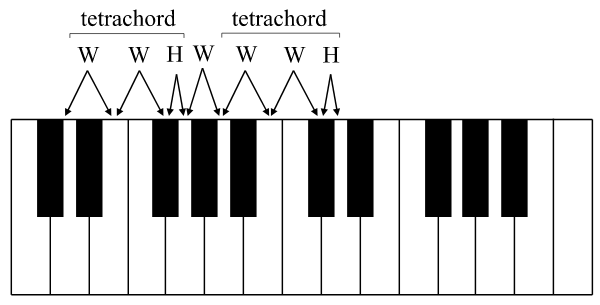
\includegraphics[width=0.6\textwidth]{img/tetrachord}
        \caption{Tetrachords in a (D) major scale}
    \end{center}
\end{figure}

A major scale uses all the 7 notes in order. No one is skipped and there are no duplicates.

\subsection{Key signatures}
There are 15 major key signatures:
\begin{itemize}
    \item 1 with no accidentals: C Major.
    \item 7 with $1$ to $7$ flats.
    \item 7 with $1$ to $7$ sharps.
\end{itemize}

\begin{figure}[h]
    \begin{center}
        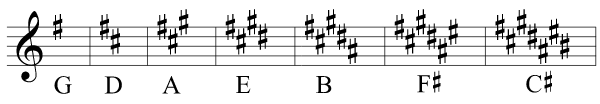
\includegraphics[width=0.8\textwidth]{img/majorsharp}
        \caption{Major key signatures (sharps)}
        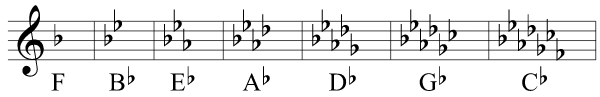
\includegraphics[width=0.8\textwidth]{img/majorflat}
        \caption{Major key signatures (flats)}
    \end{center}
\end{figure}
A key signature can be quickly identified with the following mnemonic:
\begin{itemize}
    \item With \emph{sharps}: +1 half step from the last ``sharped note''.
    \item With \emph{flats}: the second to last flat is the key (along with the flat).
\end{itemize}

\section{Minor scales}
In contrast to major scales, there are 3 different minor scales. They all follow the following formulas, while the melodic minor is only used as an \emph{ascending} scale (the \emph{descending} part is the same as the natural minor scale).
\begin{figure}
    \begin{center}
        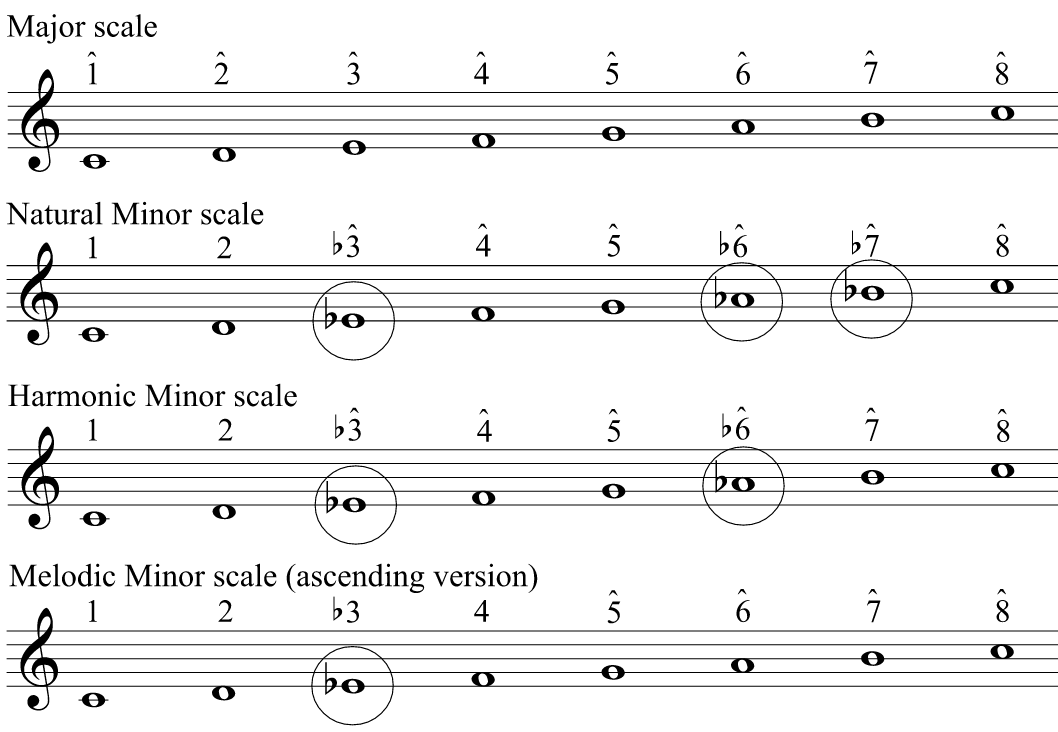
\includegraphics[width=0.8\textwidth]{img/minorscales}
        \caption{Minor scales}
    \end{center}
\end{figure}

\subsection{Key signatures}
In respect to the major keys, minor keys can be derived by adding 3 flats (or subtracting sharps and adding flats if needed).

\begin{figure}
    \begin{center}
        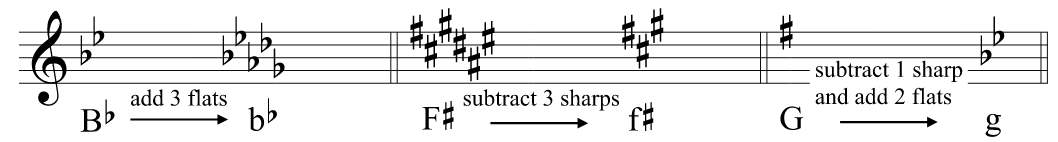
\includegraphics[width=0.8\textwidth]{img/parallel}
        \caption{Parallel relationship}
    \end{center}
\end{figure}

In doing so, the corresponding major scale will also have three of its scale degrees lowered, resulting in what is called a \textbf{parallel} minor scale.

\begin{definition}[Parallel scale relationship]
    Two major / minor scales with the same $1^{st}$ scale degree.
\end{definition}

On the other hand, if it is the key signature to be shared, then we call it a \textbf{relative} minor key.

\begin{definition}[Relative key relationship]
    Two major / minor key signatures with the same key signature.
\end{definition}

\section{Circle of fifths}
The circle of fifths is a convenient aid for the visualization of both minor and major keys and scales:
\begin{itemize}
    \item To the right, we add sharps / remove flats and we go up a $5^{th}$.
    \item To the left, we remove sharps / add flats and we go down a $5^{th}$.
\end{itemize}

\begin{figure}
    \begin{center}
        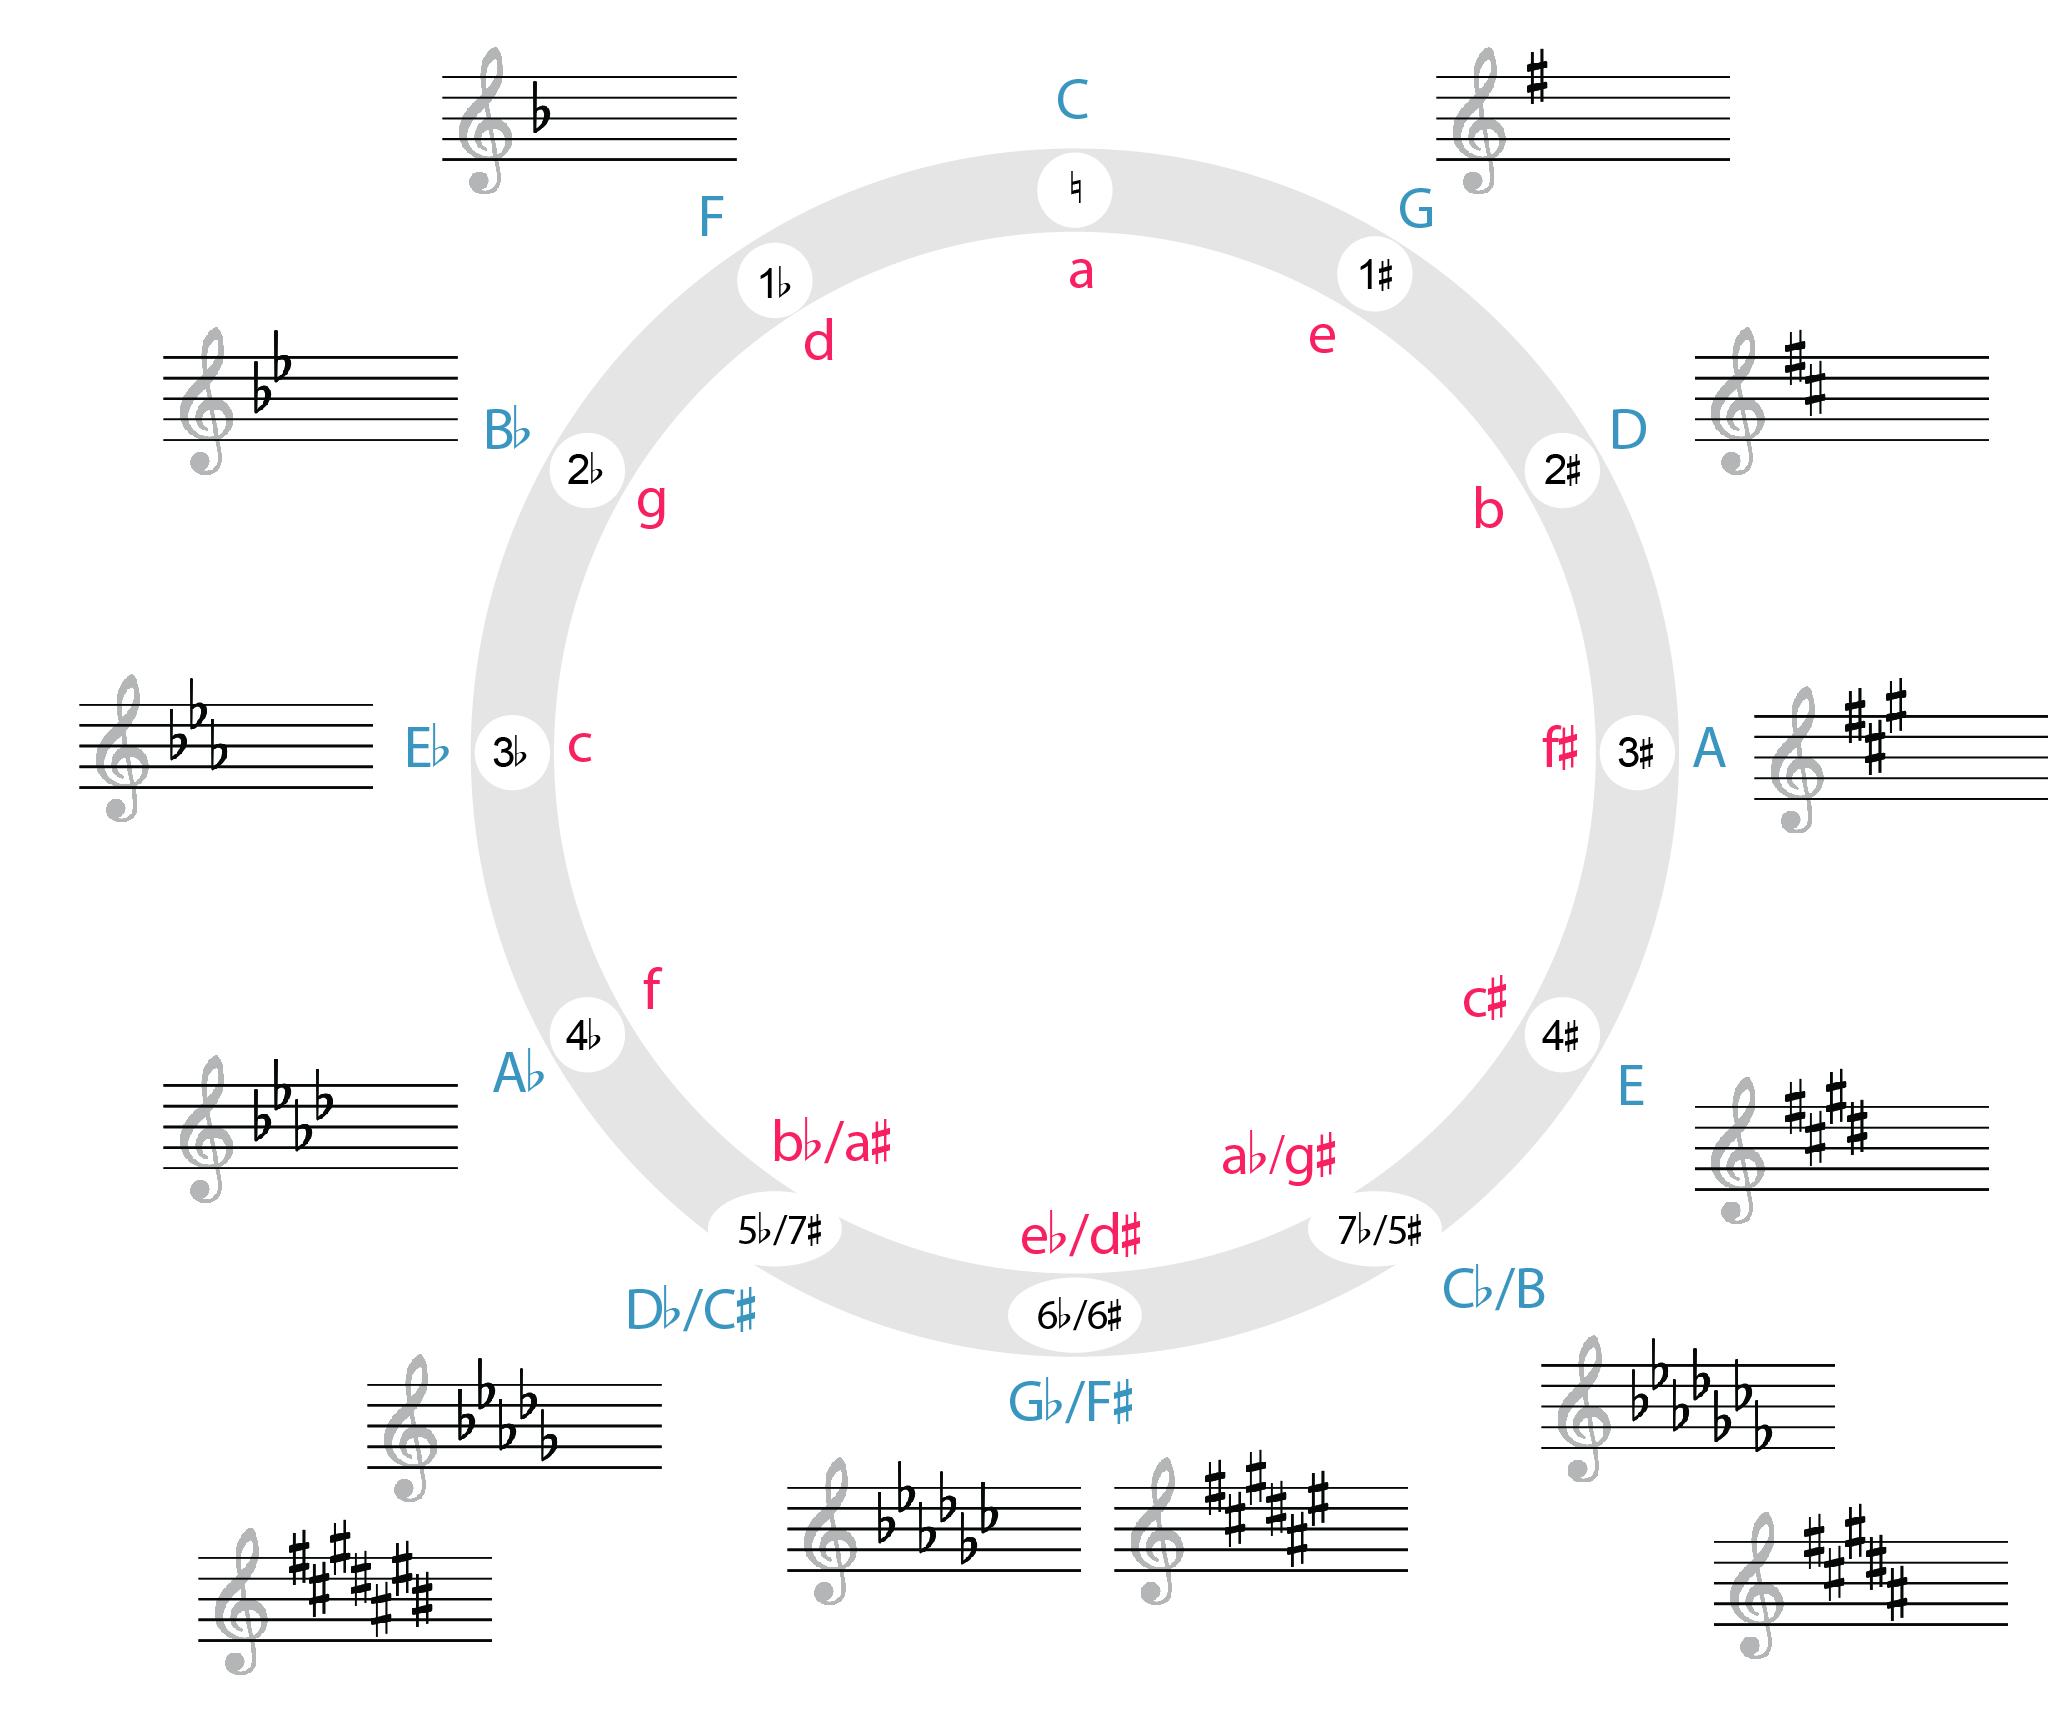
\includegraphics[width=0.8\textwidth]{img/circle}
        \caption{Circle of fifths}
    \end{center}
\end{figure}

\section{Key signature identification}
Given a piece of sheet music we can devise its key signature as follows:
\begin{enumerate}
    \item Through the number of flats / sharps we restrict ourselves to 2 key signatures: a major one and a minor one.
    \item The tonic can help us do the final discrimination. Usually the tonic note is located at the beginning / end of the piece either in the lower or upper parts.
\end{enumerate}